\documentclass{jcgt}

\setciteauthor{TODO insert your name(s) here as they should appear in the citation}
\setcitetitle{TODO insert your paper's title here without linebreaks}

% Mark submissions with the date of submission using the following line:
%\submitted{\today}

% Once an article is accepted accepted, switch to the following line and comment the preceding one. The editor will supply the argument values.
\accepted{July 4, 2013}{July 4, 2013}{July 4, 2013}{Editor Name}{2}{1}{1}{1}{2013}
\seturl{http://jcgt.org/published/0002/02/01/}




%%%%%%%%%%%%%%%%%%%%%%%%%%%%%%%%%%%%%%%%%%%%%%%%%%%%


\begin{document}

\title{JCGT Style Guidelines and\\Formatting Template}

\author
       {Roy G. Biv\\Colortech, Inc.
        \and Raymond Trace\\Graphica University
       }

% Optional teaser image
\teaser{
  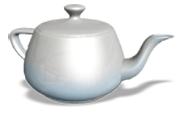
\includegraphics[width=2in]{teapot.png}
  \label{fig:teaser}
  \caption{A teapot teaser figure.}
}


\maketitle
\thispagestyle{firstpagestyle}

\begin{abstract}
\small
This document is the \textit{JCGT} formatting template \textit{and} a description of the guidelines
for  \textit{JCGT} articles.  The author names on this document are fictional and chosen to show
how to format affiliations.
\end{abstract}


%-------------------------------------------------------------------------
\section{Introduction}
\label{sec:introduction}
Documents may be typeset using any system so long as they follow the formatting
of this example, however we recommend
the use of \LaTeX\ because it simplifies typesetting.

\subsection{Related Work}
\label{sec:relatedwork}

Unless the point of the article is to provide a survey, do not survey all related work in a \textit{JCGT} article. Instead, discuss only directly relevant work against which the technique will be compared or alternatives that the reader might prefer.  There need not be an explicit related work section, however the introduction should provide enough information for the reader to know why he or she might prefer this technique to a previous one that is known to the community.


\section{Sections}
Divide the article into logical sections...

\subsection{Sub-section}
...and subsections.\pdfmarginpar{You can use pdfmarginpar to leave notes for your coauthors.  Please don't leave notes in the review copy.}

\subsubsection{Sub-subsections}
Use sub-subsections sparingly.

\paragraph{Paragraph.} Consider ``paragraph'' formatting as an alternative to sub-subsections.


\section{Abstract}
Briefly describe the topic, value of the technique, and major limitations in the abstract. For example,

``The CIE Lab color  space is useful for image editing operations and device-independent representation of
color.  However, most modern display  input  and  cameras  output is in the sRGB color space, as are stored images on disk.  We describe a method for
efficiently converting colors between the Lab and sRGB color spaces that requires no branches,  lookup tables, or floating-point operations.

Our 32-bit fixed-point
implementation is 30\% faster than the traditional (and floating point) method on
iPad 3 and Core i7 processors and produces provably
minimal error for 24-bit input color.  However,  unlike traditional color space
conversions, it does not generalize for conversions to and from CIE XYZ or
gamma 1.0 RGB space in the new method, and it is slower than direct floating-point
conversion on devices that do not support native integer instructions (e.g., DX9 GPUs).

The article includes C and GLSL source code adapted from the hardware accelerated path of the Colortech's commercial PaintMaster application for
both desktop and mobile platforms. ''

\section{Images}

Capture raster images at high resolution in a lossless format, such as PNG.  Vector images
can be directly incorporated in formats such as PDF; avoid rasterizing vector source diagrams
and results.  Include figures with captions as shown in Figure~\ref{fig:teapot}.

Figures should be near the text that refers to them whenever possible, and should not be
reduced to grayscale.  Encode images in the sRGB space (the default for PNG).

\begin{figure}[htb]
  \centering
   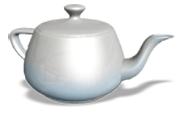
\includegraphics[width=0.5\columnwidth]{teapot.png}
   \caption{\label{fig:teapot}
     This is a teapot rendered by OpenGL with environment mapping and a Blinn-Phong BSDF.}
\end{figure}

\section{Source Code}

Format source code listings with syntax highlighting as shown in Listing~\ref{lst:hello}.  Inline
code, such as \lstinline{lerp(a, b, t)}, should also be in a fixed-width font.

\begin{lstlisting}[caption={A simple C program.}, label={lst:hello}, float]
#include <stdio.h>

/* Entry point for the program */
int main(const int argc, const char* argv[]) {

    /* Print some output */
    printf("Hello world!\n");

    return 0;
}
\end{lstlisting}

\section{Hyperlinks}
Link section, figure, table, equation, etc. reference numbers and citations to their target (the JCGT \LaTeX class automatically generates these links).

Favor standard citations over URLs whenever possible, since URLs may not stand the test of time.  When providing a URL, type the full URL text so that it is still useful in print, and create a hyperlink.  For example,
the \textit{JCGT} website is at \href{http://jcgt.org}{http://jcgt.org}.

\section{Citations and Bibliography}
Do not use citations as nouns--the text should read correctly were they omitted. For example, the following are correct:

\begin{enumerate}
\item ``The Rendering Equation \cite{Immel:1986:RMN:15886.15901,Kajiya:1986:RE:15922.15902} relates the incoming and outgoing light at a surface...''
\item ``Immel et al.'s paper~\shortcite{Immel:1986:RMN:15886.15901} uses a directional parameterization...''
\end{enumerate}

\noindent The bibliography should use ACM SIGGRAPH format.

\section{Units}
Use SI units, e.g., meters, seconds, unless there is an application-specific reason to employ a non SI-unit such as `feet'.  Units should appear in normal Roman type when in an equation, e.g.,
%
\begin{equation}
\frac{150\;\mathrm{m}}{20\;\mathrm{s}} = 75\;\mathrm{m}/\mathrm{s}
\end{equation}
%
to distinguish them from variable names.

Time performance should be measured in \textbf{time} units, e.g., ``the shader took 3.6\;s to execute on GeForce GTX 680.''  However, it is appropriate to also express values in frames per second when discussing the end-to-end performance of a complete system.  For example, the performance of a shadow algorithm implementation should be measured in milliseconds but the performance of a complete virtual reality system could be measured in frames per second instead of rendering time per frame.

\section{Mathematics}
Please use the guidelines in Table~\ref{tbl:math} for typesetting mathematics, although in some cases, domain-specific notation should overrule them.

\begin{table}[htdp]
\small
\begin{center}
\begin{tabular}{l|c}
Scalar & $x$\\
Mathematical vector & $\vec{v}$ \\
Unit vector & $\hat{\omega}$ \\
Matrix & $\mathbf{M}$ \\
Transpose & $\mathbf{M}^\transpose$\\
Inverse & $\mathbf{M}^{-1}$\\
Geometric point & $X$ \\
Set & $\mathbb{S}$ \\
Subscript expression & $h_i$ \\
Subscript name & $L_\mathrm{in}$ \\
Function & $f(x)$ \\
Named function & $\max(3, 4)$, $\operatorname{lerp}(a, b, t)$
\end{tabular}
\end{center}
\caption{Math symbol formatting guidelines.}
\label{tbl:math}
\end{table}

\noindent Equation~\ref{eqn:rendering} is an example of a numbered equation following these conventions.

\begin{equation}
L_\mathrm{o}(X, \hat{\omega}_\mathrm{o}) = L_\mathrm{e}(X, \hat{\omega}_\mathrm{o}) + \int_{\mathbf{S}^2} L_\mathrm{i}(X, \hat{\omega}_\mathrm{i}) \cdot f(\hat{\omega}_\mathrm{i}, \hat{\omega}_\mathrm{o}) \cdot |\hat{n} \cdot \hat{\omega}_\mathrm{i} |~ d\hat{\omega}_\mathrm{i}
\label{eqn:rendering}
\end{equation}

Large equations, images, and tables may exceed the regular text margins but should stop within 1.5 cm of the physical page border.

\subsection*{Acknowledgements}
Authors may provide a brief acknowledgements section if desired.

\small
\bibliographystyle{acmsiggraph}
\bibliography{paper}

\section*{Index of Supplemental Materials}
When supplemental materials such as video, data sets, and source code are provided with an article, briefly describe them by directory or filename here.

\section*{Author Contact Information}

\hspace{-2mm}\begin{tabular}{p{0.5\textwidth}p{0.5\textwidth}}
Roy G. Biv \newline
Colortech, Inc. \newline
29 Red Blvd. \newline
New York, NY 10511 \newline
\href{mailto:roy@colortech.com}{roy@colortech.com}
&

Raymond Trace \newline
Graphica University \newline
37 Rue De Lambert \newline
Paris, 75009 France \newline
\href{mailto:rtrace@graphica.edu}{rtrace@graphica.edu} \newline
\href{http://graphica.edu/~rtrace}{http://graphica.edu/\textasciitilde rtrace}

\end{tabular}


\afterdoc

\end{document}
